\documentclass[12pt,utf8,notheorems,compress,t]{beamer}
\usepackage{etex}

\usepackage{pgfpages}
\setbeameroption{show notes on second screen}
\setbeamertemplate{note page}[plain]
\newcommand{\jnote}[2]{\only<#1>{\note{\setlength\parskip{\medskipamount}\justifying\footnotesize#2\par}}}

% Workaround for the issue described at
% https://tex.stackexchange.com/questions/164406/beamer-using-href-in-notes.
\newcommand{\fixedhref}[2]{\makebox[0pt][l]{\hspace*{\paperwidth}\href{#1}{#2}}\href{#1}{#2}}

\usepackage[english]{babel}

\usepackage{graphbox}
\usepackage{mathtools}
\usepackage{booktabs}
\usepackage{stmaryrd}
\usepackage{array}
\usepackage{ragged2e}
\usepackage{multicol}
\usepackage{tabto}
\usepackage{xstring}
\usepackage{ifthen}
\usepackage[normalem]{ulem}
\usepackage[all]{xy}
\xyoption{rotate}
\usepackage{tikz}
\usetikzlibrary{calc,shapes,shapes.callouts,shapes.arrows,patterns,fit,backgrounds,decorations.pathmorphing,positioning}
\hypersetup{colorlinks=true}

\usepackage{pifont}
\newcommand{\cmark}{\ding{51}}
\newcommand{\xmark}{\ding{55}}
\DeclareSymbolFont{extraup}{U}{zavm}{m}{n}
\DeclareMathSymbol{\varheart}{\mathalpha}{extraup}{86}

\graphicspath{{images/}}

\usepackage[protrusion=true,expansion=true]{microtype}

\setlength\parskip{\medskipamount}
\setlength\parindent{0pt}

\title{Generalized spaces for constructive algebra}
\author{Ingo Blechschmidt}
\date{September 2019}

\useinnertheme[shadow=true]{rounded}
\setbeamerfont{block title}{size={}}

\useinnertheme{rectangles}

\usecolortheme{orchid}
\usecolortheme{seahorse}
\definecolor{mypurple}{RGB}{150,0,255}
\setbeamercolor{structure}{fg=mypurple}
\definecolor{myred}{RGB}{150,0,0}
\setbeamercolor*{title}{bg=myred,fg=white}
\setbeamercolor*{titlelike}{bg=myred,fg=white}
\setbeamercolor{frame}{bg=black}

\usefonttheme{serif}
\usepackage[T1]{fontenc}
\usepackage{libertine}

% lifted from https://arxiv.org/abs/1506.08870
\DeclareFontFamily{U}{min}{}
\DeclareFontShape{U}{min}{m}{n}{<-> udmj30}{}
\newcommand\yon{\!\text{\usefont{U}{min}{m}{n}\symbol{'210}}\!}

\newcommand{\A}{\mathcal{A}}
\newcommand{\B}{\mathcal{B}}
\renewcommand{\C}{\mathcal{C}}
\newcommand{\M}{\mathcal{M}}
\renewcommand{\AA}{\mathbb{A}}
\newcommand{\E}{\mathcal{E}}
\newcommand{\F}{\mathcal{F}}
\renewcommand{\G}{\mathcal{G}}
\newcommand{\J}{\mathcal{J}}
\newcommand{\GG}{\mathbb{G}}
\renewcommand{\O}{\mathcal{O}}
\newcommand{\K}{\mathcal{K}}
\newcommand{\NN}{\mathbb{N}}
\newcommand{\QQ}{\mathbb{Q}}
\newcommand{\RR}{\mathbb{R}}
\newcommand{\TT}{\mathbb{T}}
\newcommand{\PP}{\mathbb{P}}
\newcommand{\ZZ}{\mathbb{Z}}
\newcommand{\CC}{\mathbb{C}}
\renewcommand{\P}{\mathcal{P}}
\newcommand{\aaa}{\mathfrak{a}}
\newcommand{\ppp}{\mathfrak{p}}
\newcommand{\fff}{\mathfrak{f}}
\newcommand{\defeq}{\vcentcolon=}
\newcommand{\defeqv}{\vcentcolon\equiv}
\newcommand{\Sh}{\mathrm{Sh}}
\newcommand{\GL}{\mathrm{GL}}
\newcommand{\Zar}{\mathrm{Zar}}
\newcommand{\op}{\mathrm{op}}
\newcommand{\Set}{\mathrm{Set}}
\newcommand{\Eff}{\mathrm{Ef{}f}}
\newcommand{\Sch}{\mathrm{Sch}}
\newcommand{\Aff}{\mathrm{Aff}}
\newcommand{\Ring}{\mathrm{Ring}}
\newcommand{\LocRing}{\mathrm{LocRing}}
\newcommand{\LRS}{\mathrm{LRS}}
\newcommand{\Hom}{\mathrm{Hom}}
\newcommand{\Spec}{\mathrm{Spec}}
\newcommand{\lra}{\longrightarrow}
\newcommand{\RelSpec}{\operatorname{Spec}}
\renewcommand{\_}{\mathpunct{.}}
\newcommand{\?}{\,{:}\,}
\newcommand{\speak}[1]{\ulcorner\text{\textnormal{#1}}\urcorner}
\newcommand{\ul}[1]{\underline{#1}}
\newcommand{\affl}{\ensuremath{{\ul{\ensuremath{\AA}}^1}}}
\newcommand{\Ll}{\text{iff}}
\newcommand{\inv}{inv.\@}
\newcommand{\seq}[1]{\mathrel{\vdash\!\!\!_{#1}}}
\newcommand{\hg}{\mathbin{:}}  % homogeneous coordinates
\newcommand{\brak}[1]{{\llbracket{#1}\rrbracket}}
\newcommand{\pt}{\mathrm{pt}}
\newcommand{\Loc}{\mathrm{Loc}}
\newcommand{\Top}{\mathrm{Top}}

\setbeamertemplate{blocks}[rounded][shadow=false]

\newenvironment{indentblock}{%
  \list{}{\leftmargin\leftmargin}%
  \item\relax
}{%
  \endlist
}

% Adapted from https://latex.org/forum/viewtopic.php?t=2251 (Stefan Kottwitz)
\newenvironment<>{hilblock}{
  \begin{center}
    \begin{minipage}{9.05cm}
      \setlength{\textwidth}{9.05cm}
      \begin{actionenv}#1
        \def\insertblocktitle{}
        \par
        \usebeamertemplate{block begin}}{
        \par
        \usebeamertemplate{block end}
      \end{actionenv}
    \end{minipage}
  \end{center}}

\newcommand{\bignumber}[1]{
  \renewcommand{\insertenumlabel}{#1}\scalebox{1.5}{\usebeamertemplate{enumerate item}}
}
\newcommand{\bigheart}{
\includegraphics{heart}}

\newenvironment{changemargin}[2]{%
  \begin{list}{}{%
    \setlength{\topsep}{0pt}%
    \setlength{\leftmargin}{#1}%
    \setlength{\rightmargin}{#2}%
    \setlength{\listparindent}{\parindent}%
    \setlength{\itemindent}{\parindent}%
    \setlength{\parsep}{\parskip}%
  }%
  \item[]}{\end{list}}

\tikzset{
  invisible/.style={opacity=0,text opacity=0},
  visible on/.style={alt={#1{}{invisible}}},
  alt/.code args={<#1>#2#3}{%
    \alt<#1>{\pgfkeysalso{#2}}{\pgfkeysalso{#3}}}
}

\newcommand{\pointthis}[3]{%
  \tikz[remember picture,baseline]{
    \node[anchor=base,inner sep=0,outer sep=0] (#2) {#2};
    \node[visible on=#1,overlay,rectangle callout,rounded corners,callout relative pointer={(0.3cm,0.5cm)},fill=blue!20] at ($(#2.north)+(-0.1cm,-1.1cm)$) {#3};
  }%
}

\tikzset{
  invisible/.style={opacity=0,text opacity=0},
  visible on/.style={alt={#1{}{invisible}}},
  alt/.code args={<#1>#2#3}{%
    \alt<#1>{\pgfkeysalso{#2}}{\pgfkeysalso{#3}}}
}

\newcommand{\hcancel}[5]{%
  \tikz[baseline=(tocancel.base)]{
    \node[inner sep=0pt,outer sep=0pt] (tocancel) {#1};
    \draw[red!80, line width=0.4mm] ($(tocancel.south west)+(#2,#3)$) -- ($(tocancel.north east)+(#4,#5)$);
  }%
}

\newcommand{\explain}[7]{%
  \tikz[remember picture,baseline]{
    \node[anchor=base,inner sep=2pt,outer sep=0,fill=#3,rounded corners] (label) {#1};
    \node[anchor=north,visible on=<#2>,overlay,rectangle callout,rounded corners,callout
    relative pointer={(0.0cm,0.5cm)+(0.0cm,#6)},fill=#3] at ($(label.south)+(0,-0.3cm)+(#4,#5)$) {#7};
  }%
}

\newcommand{\explainstub}[2]{%
  \tikz[remember picture,baseline]{
    \node[anchor=base,inner sep=2pt,outer sep=0,fill=#2,rounded corners] (label) {#1};
  }%
}

\newcommand{\squiggly}[1]{%
  \tikz[remember picture,baseline]{
    \node[anchor=base,inner sep=0,outer sep=0] (label) {#1};
    \draw[thick,color=red!80,decoration={snake,amplitude=0.5pt,segment
    length=3pt},decorate] ($(label.south west) + (0,-2pt)$) -- ($(label.south east) + (0,-2pt)$);
  }%
}

% Adapted from https://latex.org/forum/viewtopic.php?t=2251 (Stefan Kottwitz)
\newenvironment<>{varblock}[2]{\begin{varblockextra}{#1}{#2}{}}{\end{varblockextra}}
\newenvironment<>{varblockextra}[3]{
  \begin{center}
    \begin{minipage}{#1}
      \begin{actionenv}#4
        {\centering \hil{#2}\par}
	\def\insertblocktitle{}%\centering #2}
        \def\varblockextraend{#3}
	\usebeamertemplate{block begin}}{
        \par
        \usebeamertemplate{block end}
        \varblockextraend
      \end{actionenv}
    \end{minipage}
  \end{center}}

\setbeamertemplate{headline}{%
  \begin{beamercolorbox}[wd=\paperwidth,ht=2.25ex]{}%
    \insertsectionnavigationhorizontal{\paperwidth}{}{}%
  \end{beamercolorbox}%
  \vskip0pt%
}

\setbeamertemplate{frametitle}{%
  \vskip0.4em%
  \leavevmode%
  \begin{beamercolorbox}[dp=1ex,center]{}%
  %   \usebeamercolor[fg]{item}{\textbf{{\Large \insertframetitle}}}
    \begin{tikzpicture}
      \def\R{8pt}
      \node (title) {\hil{\large\,\!\insertframetitle}};
      \begin{pgfonlayer}{background}
        \draw[decorate, very thick, draw=mypurple]
          ($(title.south west) + (\R, 0)$) arc(270:180:\R) --
          ($(title.north west) + (0, -\R)$) arc(180:90:\R) --
          ($(title.north east) + (-\R, 0)$) arc(90:0:\R) --
          ($(title.south east) + (0, \R)$) arc(0:-90:\R) --
          cycle;
      \end{pgfonlayer}
    \end{tikzpicture}
  \end{beamercolorbox}%
  \vskip-0.6em%
}

\setbeamertemplate{navigation symbols}{}

\newcounter{framenumberpreappendix}
\newcommand{\backupstart}{
  \setcounter{framenumberpreappendix}{\value{framenumber}}
}
\newcommand{\backupend}{
  \addtocounter{framenumberpreappendix}{-\value{framenumber}}
  \addtocounter{framenumber}{\value{framenumberpreappendix}}
}

\newcommand{\insertframeextra}{}
\setbeamertemplate{footline}{%
  \begin{beamercolorbox}[wd=\paperwidth,ht=2.25ex,dp=1ex,right,rightskip=1mm,leftskip=1mm]{}%
    % \inserttitle
    \hfill
    \insertframenumber\insertframeextra\,/\,\inserttotalframenumber
  \end{beamercolorbox}%
  \vskip0pt%
}


\newcommand{\hil}[1]{{\usebeamercolor[fg]{item}{\textbf{#1}}}}
\newcommand{\bad}[1]{\textcolor{red!90}{\textnormal{#1}}}

\begin{document}

\addtocounter{framenumber}{-1}

\tikzstyle{topos} = [draw=mypurple, very thick, rectangle, rounded corners, inner sep=5pt, inner ysep=10pt]
\tikzstyle{title} = [fill=mypurple, text=white]

% Taken from Todd Lehman (CC-BY-SA) at https://tex.stackexchange.com/a/44920/32372

\newcommand{\setisprime}[1]{
  % Sets \isprime based on #1.
  \ifnum#1=1 \gdef\isprime{0} \else \gdef\isprime{1} \fi
  \foreach \sip in {2, 3,5,...,#1} {
    \pgfmathparse{\sip*\sip>#1? 1:0}
    \ifthenelse{\pgfmathresult=1}{
      % Early-out if \sip^2 > #1.
      \breakforeach
    }{
      % Otherwise test if \sip divides #1.
      \pgfmathparse{Mod(#1,\sip)==0? 1:0}
      \ifthenelse{\pgfmathresult=1}{
        \gdef\isprime{0}
        \breakforeach
      }{}
    }
  }
}

\newcommand{\setxy}[1]{
  % Sets \x and \y to loction of cell #1.
  \pgfmathtruncatemacro{\x}{Mod(#1-1,\cols)}
  \pgfmathtruncatemacro{\y}{(#1-1) / \cols}
  \pgfmathtruncatemacro{\y}{\cols - 1 - \y}
  \pgfmathparse{2.5*(\x+.5)}\let\x\pgfmathresult
  \pgfmathparse{2.5*(\y+.5)}\let\y\pgfmathresult
}

\newcommand{\numlabel}[2]{
  % Draws label #2 at cell #1.
  \setxy{\n}
  \node[fill=none, text=black] at (\x,\y) {#2};
}

\newcommand{\drawpolygon}[2]{
  % Draws polygon with #2 vertexes at cell #1.
  \setxy{#1}
  \ifthenelse{#2>1}{ % Polygon must have at least 2 sides.
    \ifthenelse{#2<30}{ % Draw polygon if it has a small number of sides.
      \filldraw (\x,\y) +(90:1)
      \foreach \drawi in {1,...,#2} {-- +(\drawi/#2*360+90:1)} -- cycle;
    }{ % Else approximate with circle.
      \filldraw (\x,\y) circle(1);
    }
  }{}
}

\newcommand{\setpolygoncolor}[1]{
  % Sets color based on #1.
  \gdef\polycolor{black}
  \ifnum#1=2\gdef\polycolor{black!50!white}\fi
  \ifnum#1=3\gdef\polycolor{yellow!95!red}\fi
  \ifnum#1=5\gdef\polycolor{yellow!0!red}\fi
  \ifnum#1=7\gdef\polycolor{blue!75!green}\fi
  \ifnum#1=11\gdef\polycolor{blue!70!red}\fi
  \ifnum#1=13\gdef\polycolor{blue!40!red}\fi
  \ifnum#1=17\gdef\polycolor{green!50!blue}\fi
  \ifnum#1=19\gdef\polycolor{green!80!black}\fi
  \ifnum#1=23\gdef\polycolor{green!50!red}\fi
  \ifnum#1=29\gdef\polycolor{yellow!50!black}\fi
  \ifnum#1=31\gdef\polycolor{orange!50!black}\fi
  \ifnum#1=37\gdef\polycolor{red!50!black}\fi
  \ifnum#1=41\gdef\polycolor{purple!50!black}\fi
  \ifnum#1=43\gdef\polycolor{blue!50!black}\fi
  \ifnum#1=47\gdef\polycolor{green!50!black}\fi
  \ifnum#1=53\gdef\polycolor{white!50!black}\fi
  \ifnum#1=59\gdef\polycolor{white!50!black}\fi
  \ifnum#1=61\gdef\polycolor{white!50!black}\fi
  \ifnum#1=67\gdef\polycolor{white!50!black}\fi
}

\newcommand{\sieve}[2]{
  \def\cols{#1}
  \def\rows{#2}
  \begin{tikzpicture}[scale=.5]
  \pgfmathtruncatemacro{\nmax}{\rows * \cols}

  \foreach \n in {1,...,\nmax} {
    \begin{scope}[fill=gray, fill opacity=.05,
                  draw=gray, draw opacity=.10,
                  line width=4]
      \drawpolygon{\n}{\n}
    \end{scope}
    \setisprime{\n}
    \ifthenelse{\isprime=1}{
      \numlabel{\n}{\bf\n}
    }{
      \def\startintensity{.33}
      \def\incrintensity{.10}
      \def\intensity{\startintensity}

      \def\m{\n}
      \pgfmathtruncatemacro{\i}{\m / 2}

      % Divide \m by \i until \m is extinguished.
      % Increment \i each time it does not divide into \m.
      \whiledo{\m>1}{
        \setisprime{\i}
        \pgfmathparse{Mod(\m,\i)==0? 1:0}
        \ifthenelse{\pgfmathresult=1\and\isprime=1}{
          \setpolygoncolor{\i}
          \begin{scope}[fill=\polycolor, fill opacity=\intensity,
                        draw=\polycolor!85!black, draw opacity=\intensity,
                        line width=\intensity*1.5]
            \drawpolygon{\n}{\i}
          \end{scope}
          \pgfmathtruncatemacro{\m}{\m / \i}
          \pgfmathparse{\intensity + \incrintensity}\let\intensity\pgfmathresult
        }{
          \pgfmathtruncatemacro{\i}{\i - 1}
          \def\intensity{\startintensity}
        }
      }
      \begin{scope}[text=black, text opacity=.5]
        \numlabel{\n}{\scriptsize\n}
      \end{scope}
    }
  }

  \end{tikzpicture}
}

%\renewcommand{\sieve}[2]{SIEVE}
%\renewcommand{\fakesieve}[2]{SIEVE}

\newcommand{\drawbox}[4]{
  \node[topos, #4] [fit = #3] (#1) {};
  \node[title] at (#1.north) {#2};
}

\newcommand{\muchstuff}{
  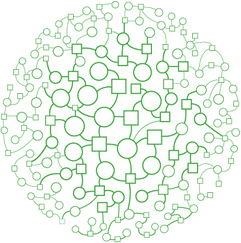
\includegraphics[height=3em]{filmat}
  \scalebox{0.5}{\sieve{14}{2}}
}

\newcommand{\muchstuffplaceholder}{
  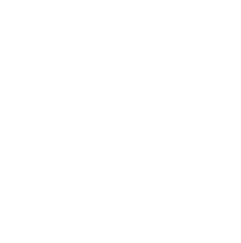
\includegraphics[height=3em]{filmat-placeholder}
  \scalebox{0.5}{\fakesieve{14}{2}}
}

\newcommand{\fewstuff}{
  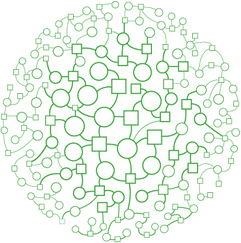
\includegraphics[height=3em]{filmat}
  \scalebox{0.5}{\sieve{7}{2}}
}

\newcommand{\threeblobs}{
  \colorbox{mypurple}{\ \ }\quad
  \colorbox{mypurple}{\ \ }\quad
  \colorbox{mypurple}{\ \ }
}

%\setbeamertemplate{headline}{\mynav{gray}{gray}{gray}}

{\usebackgroundtemplate{\begin{minipage}{\paperwidth}\vspace*{4.95cm}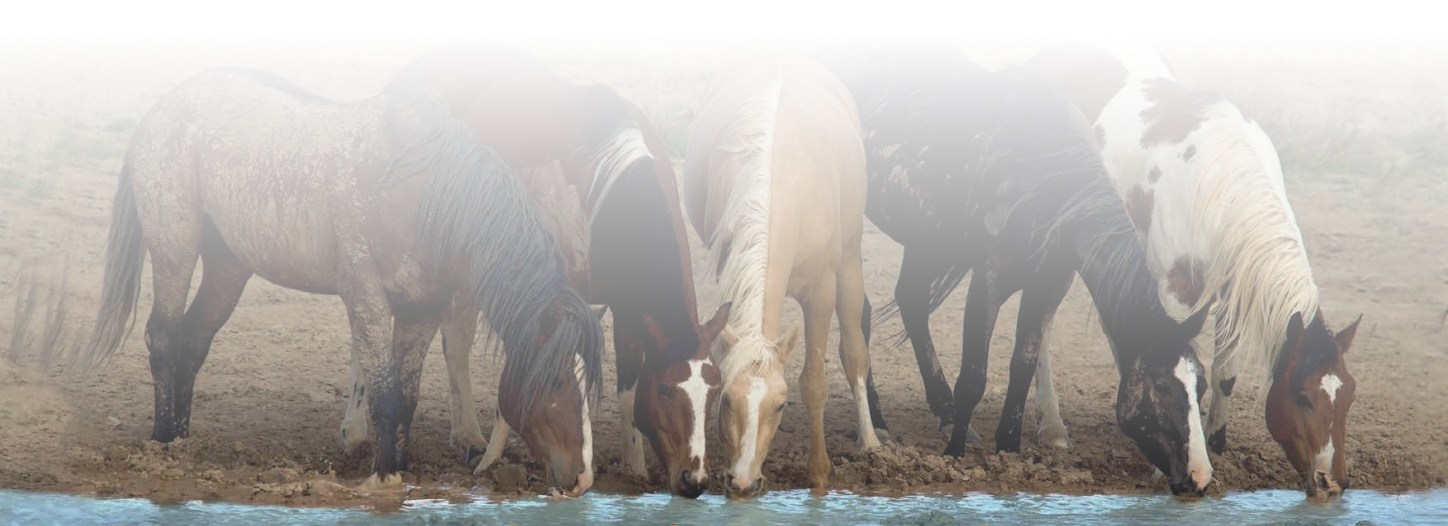
\includegraphics[width=\paperwidth]{topos-horses}\end{minipage}}
\begin{frame}[c]
  \centering

  \begin{tikzpicture}
    \def\R{8pt}
    \node (title) {\hil{\,Generalized spaces for constructive algebra\,}};
    \begin{pgfonlayer}{background}
      \draw[decorate, very thick, draw=mypurple]
        ($(title.south west) + (\R, 0)$) arc(270:180:\R) --
        ($(title.north west) + (0, -\R)$) arc(180:90:\R) --
        ($(title.north east) + (-\R, 0)$) arc(90:0:\R) --
        ($(title.south east) + (0, \R)$) arc(0:-90:\R) --
        cycle;
    \end{pgfonlayer}
  \end{tikzpicture}
  \bigskip

  \begin{columns}
    \small
    \begin{column}{0.35\textwidth}
      \centering
      \bignumber{1}
      
      \phantom{x}\hil{Locales}
      \medskip

      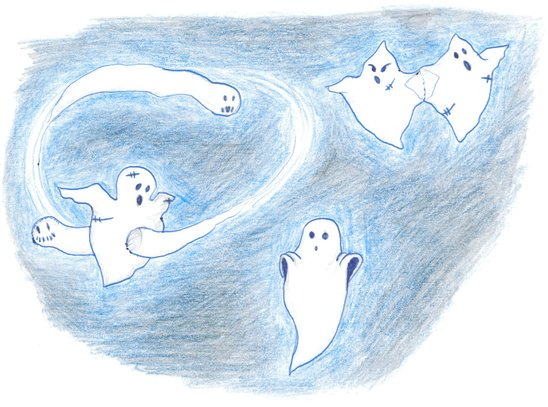
\includegraphics[height=4.5em]{phantoms.png}
    \end{column}
    \hspace*{0.5em}
    \begin{column}{0.28\textwidth}
      \centering
      \bignumber{2}

      \phantom{x}\hil{Sheaf models}
      \medskip

      \phantom{x}\!\!\begin{tikzpicture}
        \node (overview) {
          \scalebox{0.35}{\sieve{4}{3}}
        };
        \def\R{8pt}
        \begin{pgfonlayer}{background}
        \draw[decoration={bumps,segment length=8pt}, decorate, very thick, draw=mypurple]
          ($(overview.south west) + (\R, 0)$) arc(270:180:\R) --
          ($(overview.north west) + (0, -\R)$) arc(180:90:\R) --
          ($(overview.north east) + (-\R, 0)$) arc(90:0:\R) --
          ($(overview.south east) + (0, \R)$) arc(0:-90:\R) --
          cycle;
        \end{pgfonlayer}
      \end{tikzpicture}
    \end{column}
    \begin{column}{0.4\textwidth}
      \centering
      \bignumber{3}
      
      \hil{Constructive algebra}
      \medskip

      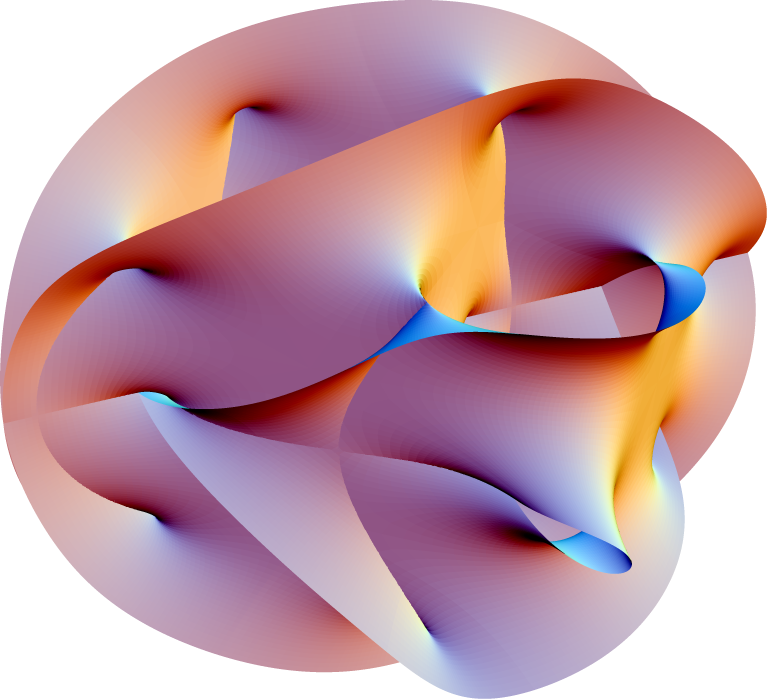
\includegraphics[height=4.5em]{calabi-yau}
    \end{column}
  \end{columns}
  \bigskip

  \scriptsize
  \textit{-- an invitation --}
  \bigskip

  Autumn school on Proof and Computation \\
  September 20th to 26th, 2019 \\
  Herrsching
  \bigskip

  Ingo Blechschmidt \\
  Università di Verona
  \par

\end{frame}}

% \begin{document}


\section{Locales}

\begin{frame}
  \centering\bigskip
  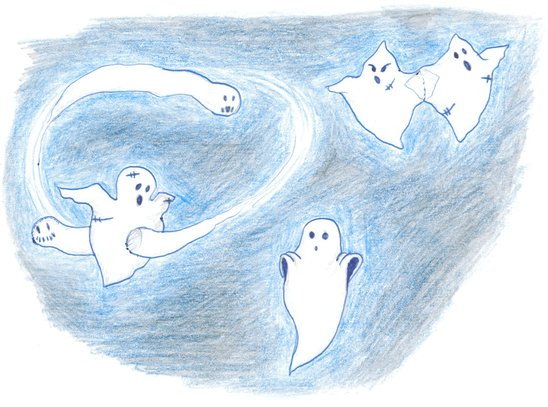
\includegraphics[height=9.5em]{phantoms}

  \large Lecture I:
  \hil{Locales}

  \normalsize

  \begin{hilblock}Locales are a kind of space in which \hil{opens} instead of
  \hil{points} are fundamental.\end{hilblock}

  \jnote{1}{
    These ``probability clouds'', replacing the reassuring material particles of
    before, remind me strangely of the elusive ``open neighborhoods'' that populate
    the topoi, like evanescent phantoms, to surround the imaginary ``points''.

    \hfill -- Alexander Grothendieck

    \bigskip
    \bigskip

    References include:
    \begin{enumerate}
      \item Peter Johnstone.
      \fixedhref{http://pointlesstopology.com/the-point-of-pointless-topology.pdf}{The point of pointless topology}, 1983.
      \item Peter Johnstone.
      \fixedhref{http://www.heldermann.de/R&E/RAE18/ctw06.pdf}{The art of
      pointless thinking: a student's guide to the category of locales}, 1990.
    \end{enumerate}

    Our metatheory is a constructive (no law of excluded middle, no choice
    principles of any kind) but impredicative (free use of the powerset axiom)
    flavor of English. The contents of this course could be formalized in the
    internal language of toposes or in~\textsc{izf}. The main ideas of this
    course are far more robust than this particular presentation, in
    particular, they can also be made sense of in a predicative setting (such
    as~\textsc{czf} or the internal language of arithmetic universes).
  }
\end{frame}

\begin{frame}{Locales in context}
  \justifying
  \textbf{Definition.} A \hil{topological space}~$X$ consists of a \hil{set of
  points} together with a set~$\O(X)$ of point sets which are deemed
  \hil{open} such that unions and finite intersections of open sets are open.
  \bigskip

  \centering\small
  \begin{tikzpicture}[sibling distance=8em, level distance=2.5em,
    every node/.style = {shape=rectangle, rounded corners,
      draw, align=center}, semithick, draw=mypurple]
    \node {euclidean spaces} [grow=up]
      child { node {metric spaces}
        child[dashed] { node [solid] {sober topological spaces}
          child[solid] { node {locales}
            child { node {toposes}
              child { node {$\infty$-toposes} } } }
          child[solid] { node {topological spaces} } } };
  \end{tikzpicture}
\end{frame}

\begin{frame}{Nontrivial spaces without points}
  The following locales don't have any points and are nontrivial:
  \begin{enumerate}
    \item the locale of surjections $\NN \twoheadrightarrow \RR$
    \item $\QQ \cap (\RR \setminus \QQ)$
    \item the pairwise intersections in the Banach--Tarski paradox
    \item Alex Simpson's locale of random binary sequences
  \end{enumerate}

  \begin{hilblock}
    Relinquishing points increases flexibility.
  \end{hilblock}

  \centering
  
\includegraphics[height=5em]{banach-tarski}

  \jnote{1}{
    The locale of surjections $\NN \twoheadrightarrow \RR$ doesn't have any
    points, but it has lots of interesting opens, such as~$U_{n,x}$, the ``open of those
    surjections~$f$ such that~$f(n) = x$. If~$x$ is a fixed real number and~$n$
    ranges over the naturals, these opens cover the full locale.

    The Banach--Tarski paradox is the unintuitive statement that a
    three-dimensional solid ball of radius~$r$ can be partitioned into six
    disjoint subsets in such a way that rearranging those subsets yields two
    solid balls of radius~$r$ each. These subsets are not measurable and
    require the axiom of choice for their construction.

    The Banach--Tarski paradox can be resolved by adopting the axiom of
    determinacy instead of the axiom of choice, which entails that all subsets
    of~$\RR^3$ are measurable, or by passing from the topological space~$\RR^3$
    to its localic cousin. The localic counterparts of the six pieces will
    still not have any points in common, but their locale-theoretic pairwise
    intersection will not be trivial.

    Tom Leinster
    \fixedhref{https://golem.ph.utexas.edu/category/2011/12/on_the_law_of_large_numbers_su.html}{published
    an accessible exposition} of the locale of random sequences at the n-category café.
  }
\end{frame}

\begin{frame}{Issues of constructivity}
  \begin{enumerate}\justifying
    \item The unit interval~$[0,1]$ is \hil{compact}.
    \bigskip

    \item \hil{The fundamental theorem of Galois theory:}
    Let~$L | k$ be a Galois extension. Then there is a bijection between
    \[ \small\begin{array}{@{}rcl@{}}
      \begin{minipage}{0.25\textwidth}\centering the intermediate extensions~$L|E|k$\end{minipage}
      &\text{and}&
      \begin{minipage}{0.33\textwidth}\centering the closed subgroups
      of~$\mathrm{Aut}_k(L)$.\end{minipage} \\
      \\
      E &\longmapsto& \{ \sigma \in \mathrm{Aut}_k(L) \,|\, \sigma|_E = \operatorname{id} \} \\
      L^H &\longmapsfrom& H
    \end{array} \]
    \medskip

    \item \hil{Gelfand duality:} The categories of
    \[ \small\begin{array}{@{}rcl@{}}
      \begin{minipage}{0.38\textwidth}\centering compact Hausdorff spaces\end{minipage}
      &\text{and}&
      \left(\begin{minipage}{0.33\textwidth}\centering commutative $C^\star$-algebras with unit\end{minipage}\right)^{\mathrm{op}} \\[1.1em]
      X &\longmapsto& \{ f : X \to \CC \,|\, \text{$f$ continuous} \}
    \end{array} \]
    are equivalent.
  \end{enumerate}

  \jnote{1}{
    By \emph{compact}, we mean any open covering has a (Kuratowski-)finite
    subcovering. The topological space~$[0,1]$ fails to be compact in some
    flavors of constructive mathematics, but the localic unit interval is
    always compact.

    In verifying the fundamental theorem of Galois theory, at some point one
    has to extend a given~$k$-homomorphism~$E \to L$ which is defined on some
    finite intermediate extension~$E$ to~$L$. One-step extensions to larger
    intermediate extensions are no problem, but extending to all of~$L$
    requires some form of choice. By passing from the topological Galois group
    to its localic group, this issue vanishes. References include the papers
    \fixedhref{https://core.ac.uk/download/pdf/82660137.pdf}{Galois theory in a topos} and
    \fixedhref{http://www.numdam.org/article/CTGDC_1981__22_1_61_0.pdf}{Localic groups} by Gavin Wraith.
    Olivia Caramello's paper
    \fixedhref{https://arxiv.org/abs/1301.0300}{Topological galois theory} is
    also relevant.

    A similar issue arises with Gelfand duality. A fully constructive treatment
    is possible by passing from compact Hausdorff (topological) spaces to
    completely regular locales. This treatment unlocks the Bohr topos approach
    to quantum mechanics.
  }
\end{frame}

\begin{frame}{Localic basics}
  \justifying
  \textbf{Definition.} A \hil{topological space}~$X$ consists of a \hil{set of
  points} together with a set~$\O(X)$ of point sets which are deemed
  \hil{open} such that unions and finite intersections of open sets are open.

  \textbf{Observation.} The partial order~$\O(X)$ of open sets has
  \[ \small\begin{array}{@{}ccc@{}}
    \text{arbitrary joins}
    &\text{and}&
    \text{finite meets}, \\
    \bigvee && \wedge
  \end{array} \]
  and finite meets distribute over arbitrary joins:
  \[ U \wedge \bigvee_i V_i = \bigvee_i (U \wedge V_i). \]
  \vspace*{-1.2em}
  \pause

  \textbf{Definition.} A \hil{frame} is a partial order with arbitrary joins
  and finite meets such that the distributive law holds.

  \textbf{Definition.} A \hil{locale}~$X$ is given by a \hil{frame~$\O(X)$ of opens}.

  \jnote{2}{
    \textbf{Example.} Any topological space~$Y$ induces a locale~$L(Y)$ by
    setting~$\O(L(Y)) \defeq \O(Y)$.

    \textbf{Example.} The \emph{one-point locale}~$\pt$ is the locale induced
    by the one-point topological space~$\{\heartsuit\}$. Its frame of opens is
    the powerset of~$\{\heartsuit\}$, also known as the set~$\Omega$ of truth
    values. Its least element is~$\bot = \emptyset$ and its largest element
    is~$\top = \{\heartsuit\}$.

    \textbf{Definition.} A \emph{frame homomorphism}~$L \to L'$ is a monotone
    map~$L \to L'$ which preserves arbitrary joins and finite meets.

    \textbf{Example.} A continuous map~$f : Y \to Y'$ induces a frame
    homomorphism~$\O(Y') \to \O(Y)$ by mapping~$U \mapsto f^{-1}[U]$.

    \textbf{Definition.} A \emph{locale morphism}~$X \to X'$ is given by a
    frame homomorphism~$\O(X') \to \O(X)$.

    \textbf{Example.} A continuous map~$Y \to Y'$ induces a locale
    morphism~$L(Y) \to L(Y')$ in the same direction.

    \textbf{Definition.} A \emph{point} of a locale~$X$ is a locale
    morphism~$\pt \to X$, or equivalently a completely prime filter of~$\O(X)$.
    (A frame morphism~$\alpha : \O(X) \to \Omega$ gives rise to the completely prime
    filter~$F \defeq \{ u \in \O(X) \,|\, \alpha(u) = \top \}$.)
  }

  \jnote{3}{
    The set of points of a locale can be made into a topological space, giving
    rise to a functor~$\pt : \Loc \to \Top$. This functor is right adjoint
    to~$L$. A locale~$X$ is \emph{spatial} iff the canonical
    morphism~$L(\pt(X)) \to X$ is an isomorphism, and a topological space~$Y$
    is \emph{sober} iff the canonical morphism~$Y \to \pt(L(Y))$ is a
    homeomorphism.
  }
\end{frame}


\section{Sheaf models}

\begin{frame}
  \centering\bigskip
  \begin{tikzpicture}
    \node (overview) {
      \scalebox{1.00}{\sieve{4}{3}}
    };
    \def\R{8pt}
    \begin{pgfonlayer}{background}
    \draw[decoration={bumps,segment length=8pt}, decorate, very thick, draw=mypurple]
      ($(overview.south west) + (\R, 0)$) arc(270:180:\R) --
      ($(overview.north west) + (0, -\R)$) arc(180:90:\R) --
      ($(overview.north east) + (-\R, 0)$) arc(90:0:\R) --
      ($(overview.south east) + (0, \R)$) arc(0:-90:\R) --
      cycle;
    \end{pgfonlayer}
  \end{tikzpicture}

  \large Lecture II:
  \hil{Sheaf models}

  \normalsize
\end{frame}

\begin{frame}{Locales presented by theories}
  \justifying
  \textbf{Definition.} A \hil{geometric signature} consists of
  \begin{enumerate}
    \item a set of sorts: $X$, $Y$, $Z$, \ldots
    \item a set of function symbols: $f : X \times Y \to Z$, \ldots
    \item a set of relation symbols: $R \hookrightarrow X \times Y \times Z$, \ldots
  \end{enumerate}
  % A geometric signature is \hil{propositional} iff its set
  % of sorts is empty.
  A \hil{geometric theory}~$\TT$ over a geometric
  signature~$\Sigma$ consists of a set of axioms (geometric sequents
  over~$\Sigma$).

  \only<1>{
    \textbf{Examples.}
    \begin{enumerate}
      \item the theory of rings
      \item the theory of surjections~$\NN \twoheadrightarrow \RR$
      \item the theory of Dedekind cuts
    \end{enumerate}
  }
  \pause

  \textbf{Definition.} A \hil{set-based model}~$M$ of a theory~$\TT$ consists of
  \begin{enumerate}
    \item a set~$\brak{X}$ for each sort~$X$,
    \item a function~$\brak{f} : \brak{X_1} \times \cdots \times \brak{X_n} \to
    \brak{Y}$ for \\
    each function symbol~$f : X_1 \times \cdots \times X_n \to
    Y$, and
    \item a relation~$\brak{R} \subseteq \brak{X_1} \times \cdots \times
    \brak{X_n}$ for \\
    each relation symbol~$R \hookrightarrow X_1 \times \cdots \times X_n$
  \end{enumerate}
  such that~$M$ validates the axioms of~$\TT$.
\end{frame}

\end{document}


% Grothendieck quote for the title picture:
%
% Ces “nuages probabilistes”, remplaçant les rassurantes particules matérielles
% d’antan, me rappellent étrangement les élusifs “voisinages ouverts” qui
% peuplent les topos, tels des fantômes évanescents, pour entourer des “points”
% imaginaires, ...
%
% Diese "Wahrscheinlichkeitswolken", welche die beruhigenden materiellen
% Partikel von früher ersetzen, erinnern mich irgendwie an die flüchtigen
% "offenen Umgebungen" der Topoi -- wie dahinschwindende Phantome, um
% die fiktiven "Punkte" zu umgeben, ...
%
% These “probability clouds”, replacing the reassuring material particles of
% before, remind me strangely of the elusive “open neighborhoods” that populate
% the topoi, like evanescent phantoms, to surround the imaginary “points”.
